% !TEX root = ../thesis-example.tex
%
\chapter{Introduction et Contexte -- Géométrie digitale et projet digitalSnow}
\label{sec:introduction}

\cleanchapterquote{We have seen that computer programming is an art, because it applies accumulated knowledge to the world, because it requires skill and ingenuity, and especially because it produces objects of beauty.}{Jean-Claude Vandamme}{Ma vie, mon œuvre.}

\setcounter{minitocdepth}{3}
\minitoc

\newpage

Depuis quelques années, nous vivons dans un monde entouré en permanence de
\colorize{données digitales}. Il ne passe pas un jour sans que nous ne soyons
bombardés de pixels, que ce soit sur les téléphones portables, les écrans
publicitaires animés, ou peut-être même actuellement si vous lisez ce document
sur un écran. Les applications sont variés et en nombre. Dans l'imagerie
médical, dans la sauvegarde du patrimoine culturel, dans la compréhension du
monde vivant, il n'est pas rare de récolter et stocker des données digitales.
Ces données brutes nécessitent des algorithmes pour les comprendre, les analyser
et en extraire des informations pertinentes.

\begin{figure}[t]
    \begin{center}
      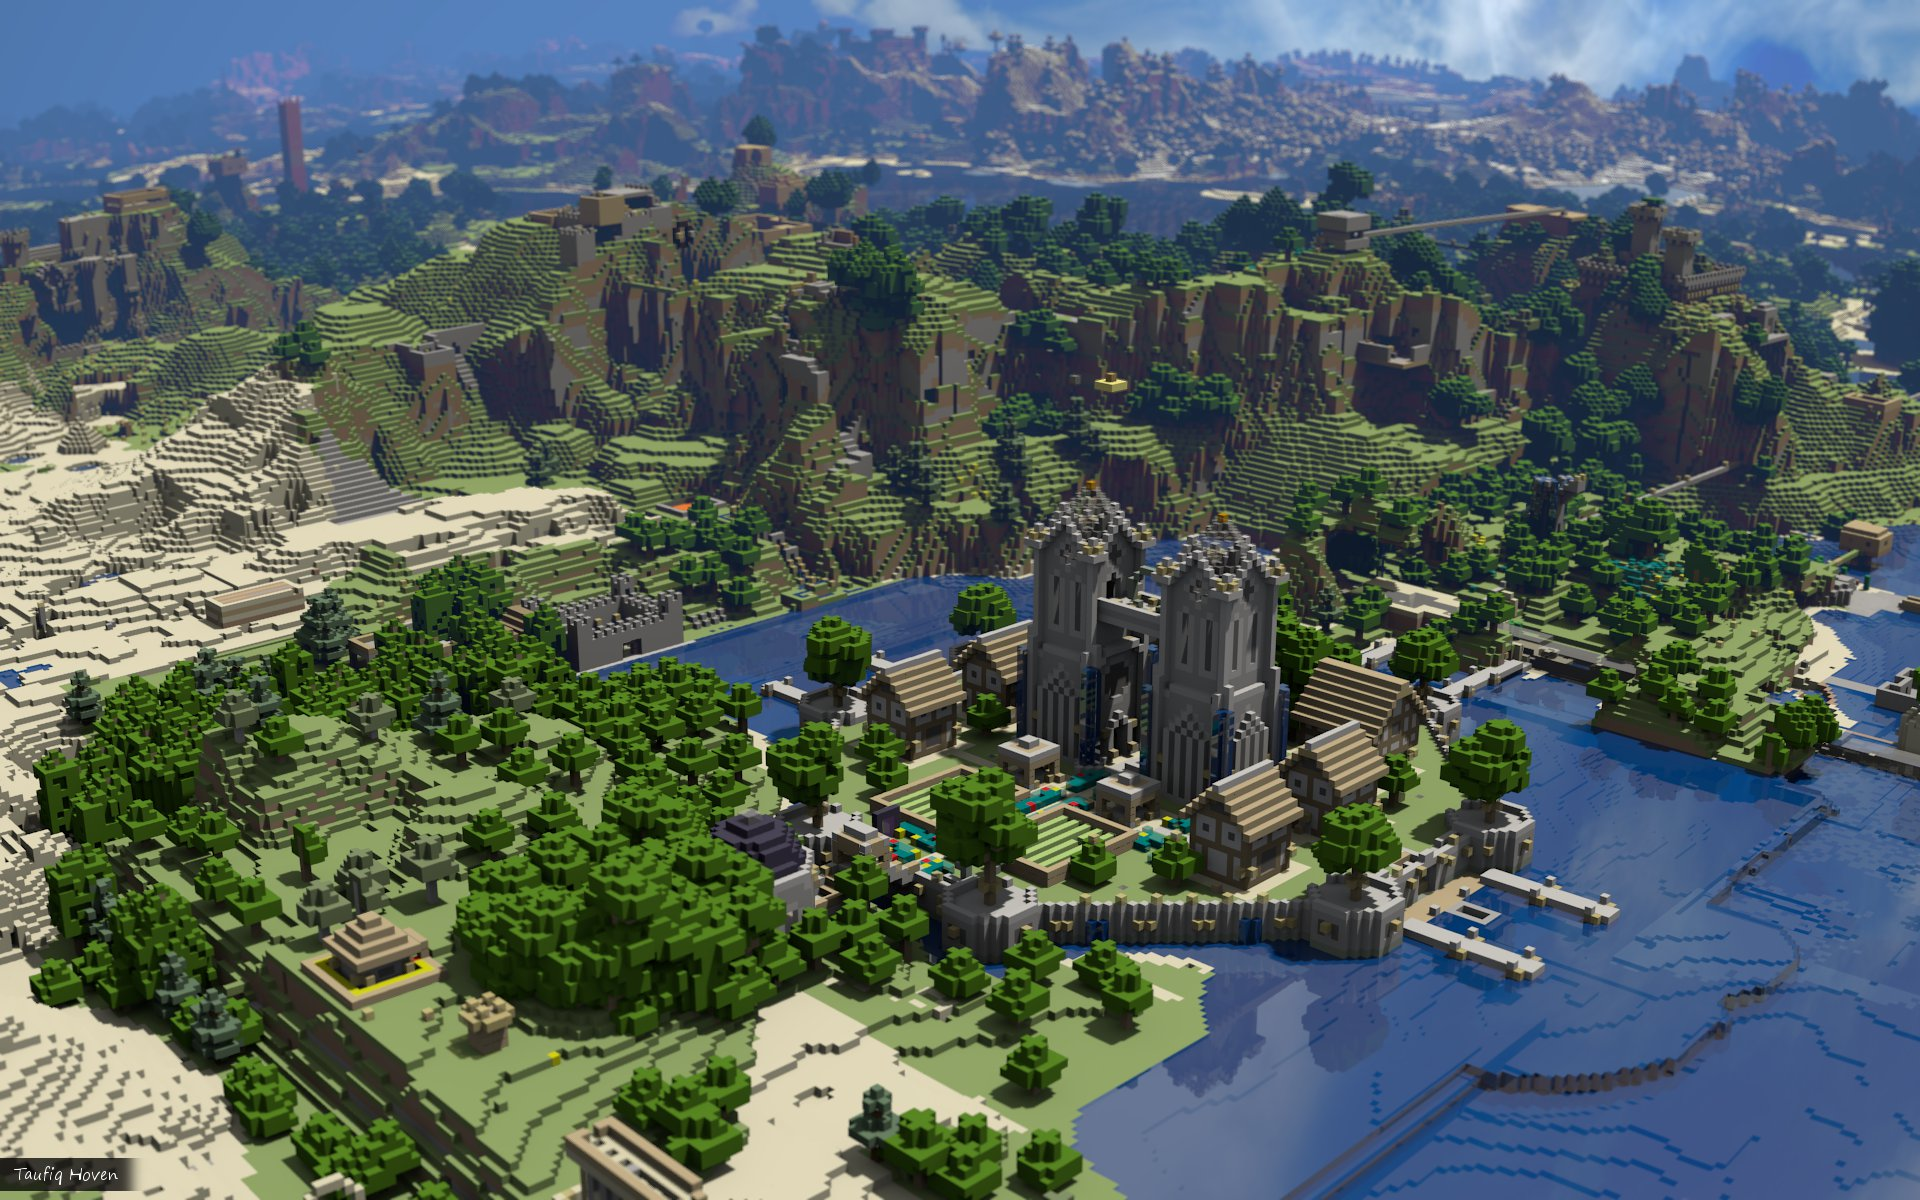
\includegraphics[width=14cm]{images/Introduction/minecraft-beautiful}
    \end{center}
    \caption{\textsc{Minecraft}, sorti en 2011 sur PC et plus tard sur consoles, représente un monde entièrement en voxels.}
    \label{fig:minecraft}
\end{figure}

Un autre domaine en plein essort fait le pari des données digitales : le jeu
vidéo. Certains moteurs de jeux ont fait le choix de basculer dans un
environnement entièrement digital. L'exemple de jeu le plus connu est
probablement \textsc{Minecraft}, sorti en 2011 sur PC : le joueur interagit avec
un monde entièrement voxelique et permet de le modifier à sa guise (\RefFigure{fig:minecraft}). Un autre
moteur comment à prendre sérieusement de l'ampleur : \textsc{Atomontage Engine}.
Celui-ci propose de modéliser entièrement l'environnement en voxel et fait un
post-traitement sur les données digitales afin d'avoir l'impression d'être sur
des données continues.

Ces données digitales sont l'objet de recherches intenses, même si le domaine
reste relativement jeune.

La géométrie discrète n'est pas seulement l'étude d'objets du monde réel dans
l'espace digital, mais également l'étude de l'objet digital lui même. Ainsi,
sous l'impulsion de Jean-Pierre \textsc{Reveillès} dès 1988, la géométrie
arithmétique s'intéresse aux droites, cercles non plus le produit d’un
algorithme de tracé mais définis intrinsèquement, sans l’être par approximation
du continu.

En 2000, durant l'école d'hiver « Digital and Image Geometry » en Allemagne, une
liste de « problèmes ouverts » en géométrie et en topologie digitale a été
dressé \cite{Klette2000OpenProblems} afin d'orienter les recherches dans le
domaines pour les années à venir. Depuis, dans cette liste beaucoup de réponses
ont été apportées. Mais on y trouve par exemple le problème « Algorithmes
d'estimation et preuves de convergence asymptotique ». Déjà à l'époque cela
représentait un problème important pouvant faire avancer le domaine de la
géométrie digitale.
